% vim: set textwidth=78 autoindent:

\subsection{Interpolation Plugin}

% when the revision of a section has been finalized, 
% comment out the following line:
%\updatedisclaimer

Il plugin di interpolazione permette d'interpolare un un layer raster TIN o IDW a partire da un layer vettoriale caricato in QGIS. È molto semplice da maneggiare e fornisce le funzionalià mostrate in Figura \ref{fig:interpolation_dialog}.

\begin{itemize}
\item \textbf{Layer vettoriale in input}: Seleziona il layer vettoriale caricato in QGIS.
\item \textbf{Attributo di interpolazione}: Seleziona la colonna attributo usata per l'interpolazione o abilita la casella \checkbox{Usa Coordinata -Z}.
\item \textbf{Metodo di interpolazione}: Seleziona il metodo di interpolazione \selectstring{Interpolazione triangolare (TIN)}{\ldots} o \selectstring{Distanza Inversa Ponderata (IDW)}{\ldots}.
\item \textbf{Numero di colonne/righe}: definisce il numero per il file raster in output
\item \textbf{Output file}: Definisce un nome per il file raster in output
\end{itemize}

\begin{figure}[ht]
   \begin{center}
   \caption{Plugin di interpolazione\nixcaption}\label{fig:interpolation_dialog}\smallskip
   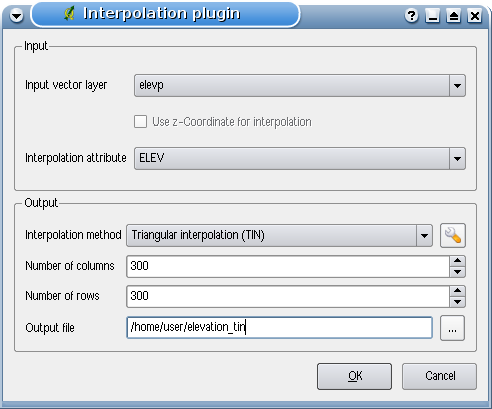
\includegraphics[clip=true, width=9cm]{interpolate_dialog}
\end{center}  
\end{figure}

\begin{enumerate}
  \item Avviare QGIS e caricare la \filename{elevp.csv} tabella CSV con i punti elevazione in QGIS usando il plugin di testo delimitato come descritto nella Sezione \ref{label_dltext}.ranslation for 
  \item Caricare il plugin di Interpolazione nel Gestore dei Plugin (see Section 
  \ref{sec:load_core_plugin}) e premere il pulsante \toolbtntwo{interpolation}{Interpolazione} che appare nella barra menu strumenti in QGIS. la finestra di dialogo del plugin di Interpolazione appare come in Figura \ref{fig:interpolation_dialog}.
  \item Selezionare \selectstring{elevp}{\ldots} come vettore di input e la colonna \filename{ELEV} per interpolazione.
  \item Selezionare \selectstring{Interpolazione triangolare}{\ldots} come metodo di interpolazione, definire 
  3663 colonne e 1964 righe (questo è equivalente ad una risoluzione pixel di 1000 metri) come nome del file raster di output \filename{elevation\_tin}.
  \item Premere \button{Ok}.
  \item Premere due volte \filename{elevation\_tin} nella legenda della mappa per aprire la finestra di dialogo Proprietà del Layer Raster e selezionare \selectstring{Pseudocolor}{\ldots} come mappa di colore nella scheda \tab{Simbologia}. Oppure 
  si può definire una nuova tabella di colori come descritto nella Sezione \ref{label_rasterprop}.
\end{enumerate}

Nella Figura \ref{fig:interpolation_idw} si vede il risultato di una interpolazione IDW con una risoluzione 366 colonne x 196 righe (10 km) per i dati \filename{elevp.csv} visualizzati usando la tabella di colore Pseudocolor. L'elaborazione impiega circa un paio di minuti, sebbene i dati riguardano soltanto la parte nord dell'Alaska.

%\begin{figure}[ht]
%   \begin{center}
%   \caption{Interpolazione di dati elevp usando il metodo IDW \nixcaption}\label{fig:interpolation_idw}\smallskip
%   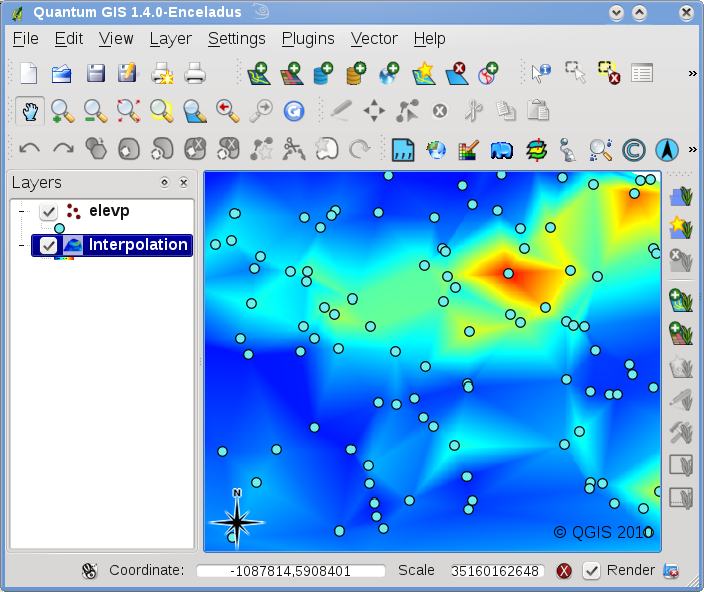
\includegraphics[clip=true, width=\textwidth]{interpolate_idw}
%\end{center}  
%\end{figure}

\newpage



